\section{Netzwerk-Applikation (APP-Layer)}

\subsection{Network Address Translation (NAT)}

Als Antwort auf das Ausgehen der IP Adressen. Verletzt grundsätzlich aber
OSI-Modell weil höhere Schicht die untere modifiziert. \textcolor{red}{Durch die
Änderung der IP-Adresse \& Port muss auch die Prüfsumme angepasst werden.}
Daten die auf einer tieferen schicht verschlüsselt werden würden Probleme bereiten.

\subsubsection{Port-basiertes NAT}
\begin{itemize}
    \item Alle Hosts des privaten 192.168.0.0/8 Netz verwenden 192.168.0.1 
        als Default-Gateway
    \item NAT-Gateway ersetzt die lokalen IP-Adressen(192.168.0.*/8) ausgehender 
        Pakete durch die eigene globale Adresse
    \item ersetzt Transport-Layer source port durch eine eindeutige freie Portnummer
    \item speichert Info welcher Host+Port auf welchen Port übersetzt wurde
    \item eingehende Pakete auf diesen Ports werden entsprechend wieder weitergeleitet
    \item[+/-] Vorteil: agiert automatisch als Firewall da eingehende Pakete nur 
        möglich sind wenn die Verbindung vom lokalen Host innitiert wurde.
    \item[+/-] auch Nachteil: eine Website auf einem lokalen Host wäre so ohne weiteres
        nicht erreichbar $\rightarrow$ gelöst durch statisches Port-basiertes NAT
    \item[-] Nachteil: limitiert auf die anzahl Ports (16-Bits also ok)
\end{itemize}


\subsubsection{statisches Port-basiertes NAT}

In der Datenbank des Gateway werden zusätzlich statische Einträge hinterlegt 
die einen Host+Port auf einen eingehenden Port mappen. Einzelne Hosts können so
über einen bestimmten Port wieder ausserhalb des lokalen Netz angesprochen werden.


\subsection{Domain Name System (DNS)}

Eine verteilte hierarchische Verzeichnisstruktur (Baum) um
Hosts innerhalb eines Domain Name Space namen zu vergeben und diese aufzulösen.

\begin{itemize}
    \item verwendet Port 53 (UDP)
	\item der Fully Qualified Domain Name (\textcolor{blue}{FQDN}) muss eindeutig
	      sein $\rightarrow$ a.b. \& a.c. ist OK obwohl 2 Hosts ''a'' heissen aber es kann nicht
	      nur ein ''a'' unter ''b'' existieren
\end{itemize}

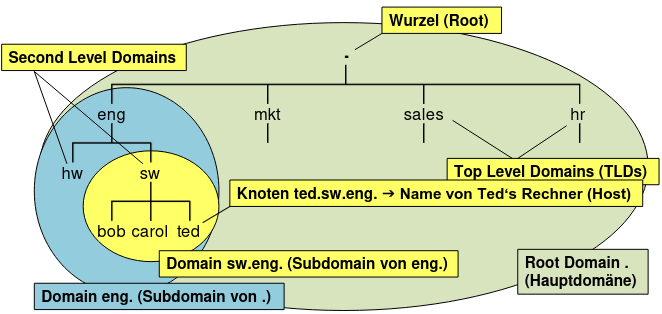
\includegraphics[width=\linewidth]{app-dns-struct}

\subsubsection{Name Server}

\begin{itemize}
    \item meist für eine Zone (eigen administrierter subtree) verantwortlich.
    \item kennt IP Adressen...
        \begin{itemize}
            \item zu Hostnamen in der Zone
            \item von Nameserver in Subdomänen (falls nicht in eigener Zone)
            \item von Root und TLD Name Server für beliebige Abfragen
        \end{itemize}
    \item für Redundanz min. 2 pro Zone
\end{itemize}


\subsubsection{DNS Abfragen}

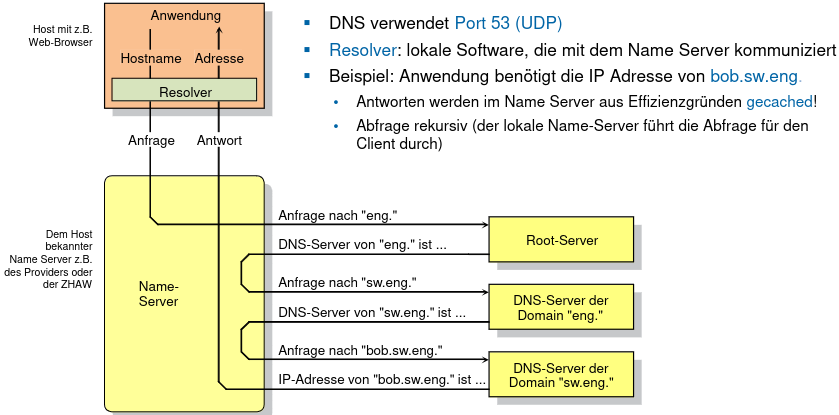
\includegraphics[width=\linewidth]{app-dns-query-ex}


\subsubsection{DNS Record Types}
\begin{description}
    \item[A] IPv4 Adresse des gesuchten Host 
    \item[AAAA] IPv6 Adresse des gesuchten Host 
    \item[MX] Mail Exchange(Server)
    \item[NS] Name Server (Namen des Server für eine Zone)
    \item[CNAME] Canonical Name: Alias für anderen Host
    \item[TXT] Text Record, in Antworten für verschiedenste Angaben verwendet
\end{description}












\subsection{Dynamic Host Configuration Protocol (DHCP)}




\subsection{Trivial File Transfer Protocol (TFTP)}




\subsection{Network Address Translation (NAT)}




\subsection{Email (SMTP, POP)}




\subsection{Hypertext Transfer Protocol}


